\documentclass[conference,compsoc]{IEEEtran}

% *** CITATION PACKAGES ***
%
\ifCLASSOPTIONcompsoc
  % IEEE Computer Society needs nocompress option
  % requires cite.sty v4.0 or later (November 2003)
  \usepackage[nocompress]{cite}
\else
  % normal IEEE
  \usepackage{cite}
\fi

% correct bad hyphenation here
\hyphenation{op-tical net-works semi-conduc-tor}


\usepackage{url}
\usepackage{adjustbox}
\usepackage{graphicx}
\usepackage{caption}
\usepackage{subcaption}
\usepackage{xcolor}
\usepackage{colortbl}
\usepackage{multirow}
\usepackage[hidelinks]{hyperref}
\usepackage[nolist]{acronym}
\usepackage{amssymb}
\usepackage{blindtext}
\usepackage{enumitem}
\usepackage{makecell}
\usepackage{listing}
\usepackage{tabularx}
\usepackage{enumitem} % Add labels for RQs defined in enumerated list
\usepackage{amsmath}
\usepackage{balance}
\usepackage{tcolorbox} % for RQ answer boxes

%% Tikz
\usepackage{tikz}
\usetikzlibrary{positioning, fit} % positioning enables relative positions in tikz, fit enable to create groups of nodes
\usepackage{tikzscale}
\usepackage{pgfplots}
\DeclareUnicodeCharacter{2212}{−}
\usepgfplotslibrary{groupplots,dateplot}
\usetikzlibrary{patterns,shapes.arrows}
\pgfplotsset{compat=newest}

%% Listings
\RequirePackage{listings}
\lstdefinelanguage{Golang}%
    {morekeywords=[1]{package,import,func,type,struct,return,defer,panic,%
    recover,select,var,const,iota,},%
    morekeywords=[2]{string,uint,uint8,uint16,uint32,uint64,int,int8,int16,%
    int32,int64,bool,float32,float64,complex64,complex128,byte,rune,uintptr,%
    error,interface},%
    morekeywords=[3]{map,slice,make,new,nil,len,cap,copy,close,true,false,%
    delete,append,real,imag,complex,chan,},%
    morekeywords=[4]{for,break,continue,range,go,goto,switch,case,fallthrough,if,%
    else,default,},%
    morekeywords=[5]{Println,Printf,Error,Print,},%
    sensitive=true,%
    morecomment=[l]{//},%
    morecomment=[s]{/*}{*/},%
    morestring=[b]',%
    morestring=[b]",%
    morestring=[s]{`}{`},%
}
\lstset{
    frame=none,
    rulecolor=\color{red},
    basicstyle=\footnotesize,
    keywordstyle=\color{blue},
    numbers=left,
    numbersep=5pt,
    showstringspaces=false,
    stringstyle=\color{darkgreen},
    tabsize=4,
    language=Golang,
    xleftmargin=17pt,
    framexleftmargin=27pt,
    framexrightmargin=5pt,
    framexbottommargin=4pt,
    breaklines=true,
    postbreak=\mbox{\textcolor{red}{$\hookrightarrow$}\space},
}

\definecolor{verylightgray}{RGB}{240,240,240}
\definecolor{darkgreen}{RGB}{20, 150, 20}
\definecolor{fuchsia}{rgb}{1.0, 0.0, 1.0}
\newcommand{\toolUsage}{\textit{go-geiger}}
\newcommand{\toolSA}{\textit{go-safer}}
\newcommand{\unsafe}{\textit{unsafe}}

\newcommand{\projsAnalyzed}{\checkNum{343}}
\newcommand{\initalProjs}{\checkNum{500}}
\newcommand{\withoutModules}{\checkNum{150}}
\newcommand{\notCompiled}{\checkNum{7}}

\newcommand{\numberPRs}{\checkNum{14}}
\newcommand{\numberPRsMerged}{\checkNum{10}}
\newcommand{\numberBugsFixed}{\checkNum{60}}

\newcommand{\percentageProjectsWithUnsafe}{\checkNum{38 \%}}
\newcommand{\percentageDependenciesWithUnsafe}{\checkNum{87 \%}}
\newcommand{\percentageProjectsAndDependenciesUnsafe}{\checkNum{91 \%}}

\newcommand{\averageUnsafeImportDepth}{\checkNum{3.08}}
\newcommand{\stdUnsafeImportDepth}{\checkNum{1.62}}


\begin{document}
%
% paper title
% Titles are generally capitalized except for words such as a, an, and, as,
% at, but, by, for, in, nor, of, on, or, the, to and up, which are usually
% not capitalized unless they are the first or last word of the title.
% Line breaks \\ can be used within to get better formatting as desired.
% Do not put math or special symbols in the title.
%\title{A Study of Prevalence, Purpose, and Risk\\ of Unsafe Go Code in the Wild}
\title{Uncovering the Hidden Dangers: \\Finding Unsafe Go Code in the Wild}


% conference papers do not typically use \thanks and this command
% is locked out in conference mode. If really needed, such as for
% the acknowledgment of grants, issue a \IEEEoverridecommandlockouts
% after \documentclass

% for over three affiliations, or if they all won't fit within the width
% of the page (and note that there is less available width in this regard for
% compsoc conferences compared to traditional conferences), use this
% alternative format:
% 
\author{
\IEEEauthorblockN{
Johannes Lauinger\IEEEauthorrefmark{2},
Lars Baumgärtner\IEEEauthorrefmark{1}, 
Anna-Katharina Wickert\IEEEauthorrefmark{1},
Mira Mezini\IEEEauthorrefmark{1}
}
\IEEEauthorblockA{
Technische Universität Darmstadt, D-64289 Darmstadt, Germany\\
}
\IEEEauthorblockA{\IEEEauthorrefmark{1}
E-mail: \{baumgaertner, wickert, mezini\}@cs.tu-darmstadt.de \\
}
\IEEEauthorblockA{\IEEEauthorrefmark{2}
E-mail: jlauinger@seemoo.tu-darmstadt.de \\
}
}

% use for special paper notices
%\IEEEspecialpapernotice{(Invited Paper)}

% make the title area
\maketitle

% As a general rule, do not put math, special symbols or citations
% in the abstract
\begin{abstract}
The Go programming language aims to provide memory and thread safety through compile-time measures such as a strict type system that prevents invalid memory accesses. 
However, it also offers a way of circumventing this safety net through the use of the \unsafe{} package.
While there are legitimate use cases for \unsafe{}, developers must exercise caution to avoid introducing vulnerabilities like buffer overflows or memory corruption in general.
%Common uses for \unsafe{} are efficiency reasons and to create functionality of generics, which are not available in current versions of Go.
%Usages of \unsafe{} may be present not only in a project's source code, but can also be introduced through dependencies.
In this work, we present \toolUsage{}, a novel tool for Go developers to quantify \unsafe{} usages in a projects source code and all of its dependencies.
%Using \toolUsage{}, we conducted a large-scale study on the usage of \unsafe{} in the \projsAnalyzed{} most popular open-source Go projects on GitHub, including a manual analysis of \numberCodeSnippets{} code samples on how \unsafe{} is used.
Using \toolUsage{}, we conducted a study on the usage of \unsafe{} in the top 500 most popular open-source Go projects on GitHub, including a manual analysis of \numberCodeSnippets{} code samples on how \unsafe{} is used.
From the projects using Go's module system  \percentagePackagesWithUnsafe{} of the dependencies contain \unsafe{} usages. 
Of these modularized projects \percentageProjectsWithUnsafe{} contain at least one usage that is not part of the standard library, and \percentageProjectsAndDependenciesUnsafe{} of projects contain at least one \unsafe{} in the project itself or one of its transitive dependencies.
Based on the usage patterns found, we present possible exploit vectors in different scenarios. 
Finally, we present \toolSA{}, a novel static analysis tool to identify dangerous and common usage patterns that were previously undetected with existing tools.

\end{abstract}

\begin{IEEEkeywords}
Golang, Static Analysis, Memory Corruption.
\end{IEEEkeywords}

% For peer review papers, you can put extra information on the cover
% page as needed:
% \ifCLASSOPTIONpeerreview
% \begin{center} \bfseries EDICS Category: 3-BBND \end{center}
% \fi
%
% For peer review papers, this IEEEtran command inserts a page break and
% creates the second title. It will be ignored for other modes.
\IEEEpeerreviewmaketitle


\section{Introduction}
\label{sec:intro}

Programming languages with direct memory access through pointers, such as C/C++, suffer from the dangers of memory corruption, including buffer overflows \cite{alnaeli2017, larochelle2001} or \textit{use-after-free} of pointers.
Microsoft, e.g., reports that memory safety accounts for around 70\% of all their bugs\footnote{\url{https://msrc-blog.microsoft.com/2019/07/16/a-proactive-approach-to-more-secure-code/}}. 
To avoid these dangers, many programming languages, such as Java, Rust, Nim, or Google's Go, use automatic memory management and prevent using low-level memory details like pointers in favor of managed object references.
Thus, these languages are memory safe, eliminating most memory corruption bugs. 
However, there are valid use cases for such low-level features.
%Systems languages may need to enforce a specific memory layout to interact with hardware or network protocols, or developers may want to achieve high performance by reusing values in memory without the need or reallocation. 
%Another reason to interact with unmanaged memory is by calling foreign functions of, e.g., a native C library.
%This degree of control over what should happen at program execution is impossible to achieve with the safety measures in place.
%
%The adoption of memory-safe languages for different kinds of applications has been increasing significantly in the last decade. 
%
%While environments and languages such as Java, Rust, Nim or Google's Go try to eliminate many bug classes through their language design and/or runtime, they also provide, to varying degrees, escape hatches to perform potentially unsafe operations.
%if explicitly requested.
%
%To serve these needs
Safe languages therefore provide, to varying degrees, escape hatches to perform potentially unsafe operations.
Escape hatches may be used for optimization purposes, to directly access hardware, to use the foreign function interface (FFI), to access external libraries, or to circumvent limitations of the programming language. 

However, escape hatches may have severe consequences, e.g., they may introduce vulnerabilities.
This is especially problematic when \unsafe{} code blocks are introduced through third-party libraries, and thus \new{are} not directly obvious to the application developer. 
Indeed, a recent study shows that unsafe code blocks in Rust are often introduced through third-party libraries~\cite{evans2020}. 
%Not knowing about the dangers introduced through external dependencies can have severe consequences, e.g., potential vulnerabilities.
\new{Therefore}, security analysts, developers, and administrators need efficient tools to quickly evaluate potential risks in their code base but also the risks introduced by code from others.

In this paper, we investigate Go and the usage of \unsafe{} code blocks within its most popular software projects. 
We developed two specific tools for developers and security analysts.
The first one, called \toolUsage{} (Section~\ref{sec:appr:toolUsage}) analyzes a project including its dependencies for locating usages of the \unsafe{} API and scoring \unsafe{} usages in Go projects and their dependencies. 
It is intended to give a general overview of \unsafe{} usages in a project. % and in which context.

As \unsafe{} usages are benign when used correctly, safe usages of \unsafe{} exist.
\new{However, we identified several commonly used \unsafe{} patterns, e.g., to cast slices and structs, which can break memory safety mechanisms.
They introduce potential vulnerabilities, e.g., by allowing access to additional memory regions. 
We provide insights into the dangers and possible exploit vectors to these patterns, indicating the severe nature of these bugs leading to information leaks or code execution (Section~\ref{sec:appr:vulnerabilites}).
%Therefore, we developed proof-of-concepts for the identified issues, leading to information leaks or code execution.

While the Go tool chain provides a linter, called \textit{go vet}, covering invalid \unsafe{} pointer conversions, 
the linter fails to flag the potentially insecure usages. 
Thus, to support developers we implemented a second tool \toolSA{} (Section~\ref{sec:appr:toolSA}) covering two types of those.}
%However, we identified two patterns which cause potentially dangerous \unsafe{} usages
%and can break the memory safety mechanisms, e.g., by allowing access to additional memory regions via type casts.
%To identify these patterns, we implemented our second tool \toolSA{} (Section~\ref{sec:appr:toolSA}).
%It helps during application development by providing meaningful hints for these usages of \unsafe{} that were previously uncaught with existing tools.

With the help of \toolUsage{}, we performed a quantitative evaluation of the top \initalProjs{} most-starred Go projects on GitHub to see how often \unsafe{} is used in the wild (Section~\ref{sec:eval:unsafewild}). 
Including their dependencies, we analyzed more than \packagesAnalyzedRounded{} individual packages. % for usage of \unsafe{}.
We found that \percentageProjectsWithUnsafe{} of projects contain \unsafe{} usages in their direct application code, and \percentageProjectsAndDependenciesUnsafe{} of
projects contain \unsafe{} usages either in first-party or imported third-party libraries.

We also created a novel data set with \checkNum{1,400} labeled occurrences of \unsafe{}, providing insights into the motivation for introducing \unsafe{} in the source code in the first place (Section~\ref{sec:eval:labeledData}). 
\new{Finally, we used \toolSA{} to find instances of our identified dangerous usage patterns within the data set.}
So far, in the course of this work we submitted \numberPRs{} pull requests to analyzed projects and libraries, fixing over \numberBugsFixed{} individual potentially dangerous \unsafe{} usages \new{(Section~\ref{sec:discussion})}. % \new{ as presented in Section~\ref{sec:discussion}}.

In this paper, we make the following contributions:
%
\begin{itemize}
\item \toolUsage{}, a first-of-its-kind tool for detecting and scoring \unsafe{} usages in Go projects and their dependencies,
\item a novel static code analysis tool, \toolSA{}, to aid in identifying potentially problematic \unsafe{} usage patterns that were previously uncaught with existing tools,
\item a quantitative evaluation on the usage of \unsafe{} in \projsAnalyzed{} top-starred Go projects on GitHub,
\item a novel data set with \checkNum{1,400} labeled occurrences of \unsafe{}, providing insights into what is being used in real-world Go projects and for what purpose, and
\item evidence on how to exploit \unsafe{} usages in the wild.
\end{itemize}

%The paper is organized as follows:
%Section~\ref{sec:background} gives a short introduction to \unsafe{} usage in Go code.
%We discuss \unsafe{} code patterns including possible exploit vectors in Section~\ref{sec:appr}, and present the design and implementation of our tools \toolUsage{} and \toolSA{}. 
%In Section~\ref{sec:eval}, we present our study on unsafe Go code in the wild.
%Then, Section~\ref{sec:discussion} discusses our approach and the study results, including potential threads to validity.
%Section~\ref{sec:rw} discusses related work and Section~\ref{sec:concl} concludes the paper.
\section{Background}
\label{sec:background}

Programming languages that offer direct memory access through pointers, such as C, have traditionally had the problem of a number of common memory vulnerability patterns.
Common problems include buffer overflows \cite{alnaeli2017, larochelle2001} or using pointers after they have been freed.
To reduce this danger, many programming languages like Java or Python use automatic memory management and largely prevent developers from using low-level memory details like pointers in favor of managed object references.

However, there exist valid use-cases for access to such low-level aspects.
Systems languages may need to enforce a specific memory layout in order to interact with hardware or network protocols, or developers may want to achieve high performance by reusing values in memory without the need or reallocation. This degree of control over what is happening at program execution might be impossible with the safety measures in place.

Therefore, some safe languages like Go also include ways to explicitly circumvent the safety measures. The \texttt{unsafe} package in the Go standard library\footnote{\url{https://golang.org/pkg/unsafe}} is a means of doing this. It is a small package that contains three functions \texttt{Sizeof}, \texttt{Alignof}, and \texttt{Offsetof} that are all evaluated at compile time and provide access into memory alignment details of Go data types that would normally be unnecessary to know.
Furthermore, the package provides a pointer type, \texttt{unsafe.Pointer} that allows developers to avoid the restrictions that are in place for regular pointer types.
In particular, it is possible to 

\begin{itemize}
    \item cast any pointer to unsafe.Pointer,
    \item cast unsafe.Pointer to any pointer,
    \item cast unsafe.Pointer to uintptr, and
    \item cast uintptr to unsafe.Pointer
\end{itemize}

The first two rules allow casts between completely arbitrary types, and the other two allow the use of pointer arithmetic.
The usage of the \texttt{unsafe} package removes the safety net provided by the Go type system and compiler, and brings developers down to the flexibility and danger of the pointers in C.

The following two examples show how the \texttt{unsafe} package can be used in practice.
In Listing~\ref{lst:unsafe-ex-in-place-cast}, \texttt{unsafe.Pointer} is used according to rules 1 and 2 to cast the \texttt{in.Items} slice to a new type without reallocating it for efficiency reasons.
The code is taken from the Kubernetes \texttt{k8s.io/apiserver} module with minor adjustments.

\begin{lstlisting}[language=Golang, label=lst:unsafe-ex-in-place-cast, caption=In-Place Cast using the Unsafe Package]
func autoConvert(in *PolicyList, out *audit.PolicyList) error {
	// [...]
	out.Items = *(*[]audit.Policy)(unsafe.Pointer(&in.Items))
	return nil
}
\end{lstlisting}

Listing~\ref{lst:unsafe-ex-escape-analysis} shows how an \texttt{unsafe.Pointer} value can be converted to \texttt{uintptr}, a non-reference type that is large enough to store memory addresses, and back to hide it from the Go escape analysis.

\begin{lstlisting}[language=Golang, label=lst:unsafe-ex-escape-analysis, caption=Hiding a Value from Escape Analysis]
func NoEscape(p unsafe.Pointer) unsafe.Pointer {
	x := uintptr(p)
	return unsafe.Pointer(x ^ 0)
}
\end{lstlisting}

Go uses escape analysis to decide whether variables can be allocated on the stack, or need to be placed on the heap \cite{wang2020}.
Since \texttt{uintptr} values are not regarded as pointer types, storing the address of a pointer in a variable of such a type and then converting it back causes the escape analysis algorithm to miss the chain of references to the underlying value in memory, therefore Go will assume a value does not escape when it actually does, and may place it on the stack.
When developers use this pattern correctly, it can be used for improved efficiency because deallocation is faster on the stack than on the heap.
However, used incorrectly it can cause security problems as described in the next section.


% \subsection{Go Dependency Management}

%Old way: packages, Go Path

%New way: modules, registries, \textit{go.mod} file.

%Package cache, versions, bad reproducibility, relatively high error rates for dependency resolution.

\section{Approach}
\label{sec:appr}

This section describes problems with using \unsafe{} that we identified, as well as information on how to exploit these issues in the wild.
Furthermore, we present our two novel tools, \toolUsage{} and \toolSA{}, that aid in locating, evaluating and fixing potentially dangerous unsafe usages in source code.

\subsection{Usage and Security Problems}

In the following, we discuss potential threat models and exploit vectors against real-world \unsafe{} Go code.
We discuss a code pattern that is used very commonly in popular open-source Go projects as our study shows.
Listing~\ref{lst:string-to-bytes} shows how \texttt{unsafe.Pointer} is used convert a string to a \texttt{reflect.StringHeader} type.
Then, a \texttt{reflect.SliceHeader} instance is created and its fields are filled by copying the respective values from the string header.
Finally, the slice header object is converted into an actual slice of type \texttt{[]byte}.
In Go, strings are essentially read-only byte slices, and slices are represented internally by a data structure that contains its current length, allocated capacity, and memory address of the actual underlying data array.
The \texttt{reflect} header structures provide access to the internal representation.

\begin{lstlisting}[language=Golang, label=lst:string-to-bytes, caption=Common Usage of Unsafe: Conversion from String to Bytes]
func StringToBytes(s string) []byte {
	strHeader := (*reflect.StringHeader)(unsafe.Pointer(&s))
	bytesHeader := reflect.SliceHeader{
		Data: strHeader.Data,
		Cap:  strHeader.Len,
		Len:  strHeader.Len,
	}
	return *(*[]byte)(unsafe.Pointer(&bytesHeader))
}
\end{lstlisting}


\subsubsection*{Implicit Read-Only}

The conversion pattern shown in Listing~\ref{lst:string-to-bytes} is efficient as it casts between \texttt{string} and \texttt{[]byte} in-place, without the need of reallocating the slice.
Using \texttt{bytes := ([]byte)(s)} for the conversion would make the compiler allocate new memory for the slice header describing \texttt{bytes} as well as the underlying data array.
However, this pattern creates an implicitly read-only byte slice that can cause problems later on.

The Go compiler will place strings into a constant data section of the resulting binary file.
Therefore, when the binary is loaded into memory the \texttt{Data} field of the string header may contain an address that is located on a read-only memory page.
Because of this, strings are immutable by design in Go.
Mutating a string will cause a compiler error, alerting developers early in the development process that there is a problem.
However, when casting the string to a \texttt{[]byte} slice in-place, the resulting slice loses the explicit read-only property and thus the compiler will not complain about mutating this slice although the program will crash if done so.
Using this pattern therefore creates a trade-off between performance and development complexity because there are potential bugs crashing the program that can be very hard to debug if the slice resulting from this conversion gets passed around.


\subsubsection*{Garbage Collector Race}

Go uses a concurrent mark-and-sweep garbage collector to free unused memory.
It is triggered by a certain increase of heap memory usage or after some time, and runs in multiple parallel Goroutines.
The garbage collector treats pointer types, \texttt{unsafe.Pointer} values, and slice and string headers that belong to actual strings and slices as references and will mark those references as still in use, preventing them from being freed.
Importantly, \texttt{uintptr} values and string or slice headers that are created manually are not treated as references.
The last point, although documented with the \texttt{unsafe} package, is a major pitfall.
It requires that values in memory that are only reachable by converting an address stored only in a \texttt{uintptr} variable to a pointer type be treated as potentially gone.
Such cast operations create potentially dangling pointers because the memory at that address might have already been freed if the garbage collector was triggered right before the conversion.

Although not directly obvious, Listing~\ref{lst:string-to-bytes} contains such a condition.
Because the \texttt{reflect.SliceHeader} value is created as a composite literal instead of being derived from an actual slice value, its \texttt{Data} field is not treated as a reference if the garbage collector runs between lines 3 and 8, and thus the underlying data array of the resulting \texttt{[]byte} slice after the conversion might have already been collected.
This creates a potential use-after-free or buffer reuse condition that, even worse, is triggered non-deterministically when the garbage collector runs at just the right time.
Therefore, it is a race condition that can crash the program or even be an information leak vulnerability.
If the buffer is reused after being freed and the resulting slice after the cast is pointing to it, it might provide access to completely unrelated data even in concurrent Goroutines, and this has serious security implications if the resulting slice is read back to a user.

\begin{figure}[!t]
    \vspace{2mm}
    \centering
    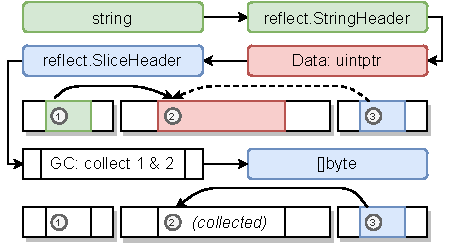
\includegraphics[width=0.4\textwidth]{gfx/figures/gcrace-vuln.pdf}
    %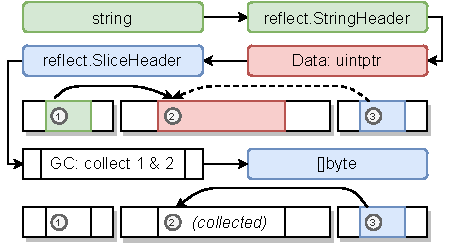
\includegraphics[width=0.48\textwidth]{gfx/figures/gcrace-vuln.pdf}
    \caption{GC race and escape analysis flaw}
    \label{fig:gcrace-vuln}
    \vspace{-8pt}
\end{figure}


Figure~\ref{fig:gcrace-vuln} shows a visualization of the casting process that leads to the problems described here.


\subsubsection*{Escape Analysis Flaw}

A third problem with the casting pattern shown in Listing~\ref{lst:string-to-bytes} is that the escape analysis algorithm can not infer a connection between the string parameter \texttt{s} and the resulting byte slice.
Although they use the same underlying data array, the algorithm misses this due to the fact that the intermediate representation as \texttt{uintptr} variable is not treated as a reference type.
This can cause the program to have undefined behavior if the returned value from the casting function is used incorrectly.

Listing~\ref{lst:escape-analysis} shows a simple program that uses the common conversion function of Listing~\ref{lst:string-to-bytes}.
In the \texttt{main} function, \texttt{GetBytes} is called which creates a string and converts it into a bytes slice using the unsafe cast.
The string is created using a \texttt{bufio} reader so that it is not constant and thus placed into the constant section of the binary, but it could also be user-provided input.
After the cast, \texttt{GetBytes} prints the resulting bytes and returns it back to \texttt{main}, which also prints the bytes.
Although one would assume that both print statements result in the string to be printed, the second one in \texttt{main} fails and prints invalid data.

\begin{lstlisting}[language=Golang, label=lst:escape-analysis, caption=Escape Analysis Flaw]
func main() {
	bytesResult := GetBytes()
	fmt.Printf("main: %s\n", bytesResult) // expected (but failed) stdout is "abcdefgh
}

func GetBytes() []byte {
	reader := bufio.NewReader(strings.NewReader("abcdefgh"))
	s, _ := reader.ReadString('\n')
	out := StringToBytes(s)
	fmt.Printf("GetBytes: %s\n", out) // expected stdout is "abcdefgh"
	return out
}
\end{lstlisting}

The reason for this is that when the string \texttt{s} is allocated in \texttt{GetBytes}, Go escape analysis will try to figure out if it escapes.
It finds that \texttt{s} is passed to \texttt{StringToBytes} and the escape analysis transitively looks into that function, where it fails to connect \texttt{s} to the returned byte slice as described above.
Therefore, escape analysis finds that \texttt{s} s does not escape in \texttt{StringToBytes}, and because it is not used after that call in \texttt{GetBytes}, the algorithm incorrectly assumes that it does not escape at all and places \texttt{s} on the stack.
When \texttt{GetBytes} prints the resulting slice, the data is still valid and the correct data is printed, but when \texttt{GetBytes} returns to \texttt{main}, its stack is destroyed.
\texttt{bytesResult} in \texttt{main} now is a dangling pointer into the former stack of \texttt{GetBytes} and therefore printing the bytes accesses invalid data.


\subsubsection*{Correct In-Place Cast}

To avoid the problems described in the previous sections, it is crucial to not create instances of \texttt{reflect.SliceHeader} and \texttt{reflect.StringHeader} from scratch, instead they must be derived from actual slices or strings.
Although this is documented with the \texttt{unsafe} package, there are many incorrect usages in the projects we analyzed.
A correct version of the in-place cast is shown in Listing~\ref{lst:correct-slice-cast}.

\begin{lstlisting}[language=Golang, label=lst:correct-slice-cast, caption=Correct In-Place String to Bytes Cast]
func StringToBytes(s string) (b []byte) {
	strHeader := (*reflect.StringHeader)(unsafe.Pointer(&s))
	bytesHeader := (*reflect.SliceHeader)(unsafe.Pointer(&b))
	bytesHeader.Data = strHeader.Data
	bytesHeader.Cap = strHeader.Len
    bytesHeader.Len = strHeader.Len
	return
}
\end{lstlisting}


\subsubsection*{Potential Code Execution}

To show further potential for real threats using \unsafe{}, we created a proof of concept for a code execution exploit using Return Oriented Programming (ROP) on a vulnerability caused by a misuse of \unsafe{}.
The vulnerability causes a buffer overflow, and since Go programs are typically statically linked with a big runtime, ASLR is not effective and there is a large number of gadgets available.
Since including the proof of concept in this paper would be too long, we put it along with other exploit demonstrations into a repository on GitHub\footnote{\url{https://github.com/jlauinger/go-unsafepointer-poc}}. 


\subsection{\toolSA{}: An Unsafe-focused Linter for Developers}

This section presents \toolSA{}, a novel static code analysis tool to find two usage patterns that were previously uncaught with existing tools.

\subsubsection*{Design}

Figure~\ref{fig:safer-architecture} shows an overview of the architecture of \toolSA{}.
\toolSA{} build upon the infrastructure provided by the Go Vet tool, which allows to add new static code analysis passes that can depend on existing ones, without having to build the CLI and output logic as well as package parsing.

\begin{figure}[!t]
    \vspace{2mm}
    \centering
    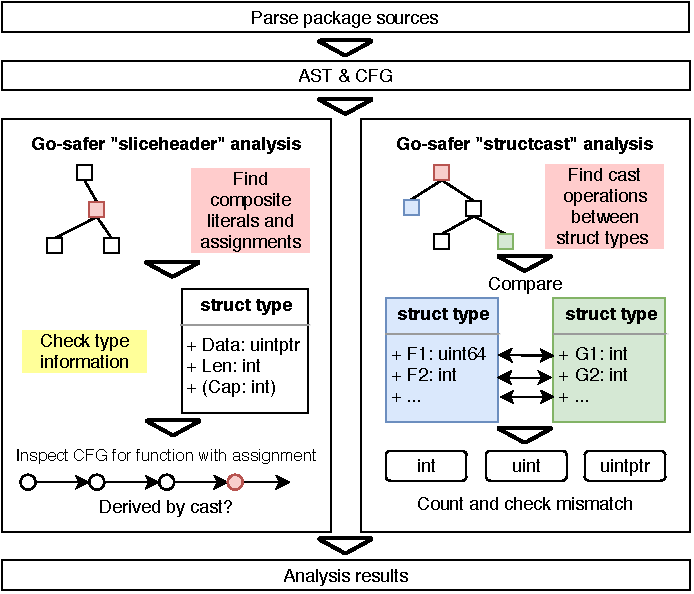
\includegraphics[width=0.48\textwidth]{gfx/figures/go-safer-architecture.pdf}
    %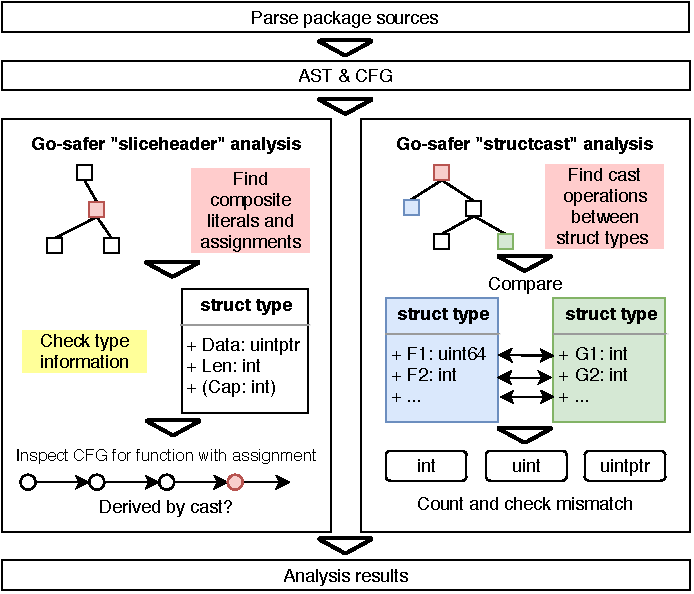
\includegraphics[width=0.45\textwidth]{gfx/figures/go-safer-architecture.pdf}
    \caption{Architecture of \toolSA{} static code analysis tool}
    \label{fig:safer-architecture}
    %\vspace{-14pt}
\end{figure}


%% put this here to manually position the figure one page earlier. Belongs to the next section (go-geiger), reposition if needed.
\begin{figure}[htp!]
    %\vspace{2mm}
    \centering
    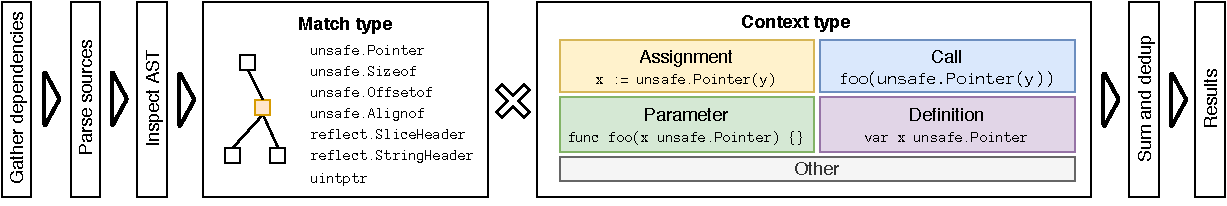
\includegraphics[width=\textwidth]{assets/figures/chapter4/go-geiger-architecture.pdf}
    \caption{Architecture of the \toolGeiger{} tool to detect unsafe usages}
    \label{fig:geiger-architecture}
    %\vspace{-10pt}
\end{figure}



\subsubsection*{Implementation}

We contribute two different novel passes: \textit{sliceheader} and \textit{structcast}.
The \textit{sliceheader} pass finds \texttt{*ast.CompositeLit} nodes in the abstract syntax tree (AST) and determines whether their type is \texttt{reflect.StringHeader}, \texttt{reflect.SliceHeader} or some derived type with the same signature.
Furthermore, it finds \texttt{*ast.AssignStmt} nodes representing assignments to variables of such types.
If it finds any, it looks up the assignment statement in the control flow graph of the corresponding function, tracks back the most recent definition of the header variable and determines whether it was derived by a cast.
If it can not certainly infer that it was in fact cast from a real slice or string, the tool will issue a warning.
The \textit{structcast} pass finds instances of in-place casts between different struct types, where the types contain an unequal amount of fields with types \texttt{int}, \texttt{uint}, or \texttt{uintptr}.
These fields have architecture-dependent sizes and offsets, and therefore casting between them might work on one architecture but break on other architectures or with different of future compilers, thus creating a risk of bugs that can crash the program or lead to invalid results on a target platform while still working fine on the developer's platform.


\subsection{\toolUsage{}: Automatic Identification of Unsafe Usage}

This section presents \toolUsage{}, a novel tool to identify and count usages of \unsafe{} in a package and its dependencies.
The project is inspired by \textit{Cargo Geiger}\footnote{\url{https://github.com/rust-secure-code/cargo-geiger}}, a similar tool for detecting unsafe code blocks in Rust programs.

\subsubsection*{Design}

Figure~\ref{fig:geiger-architecture} shows an overview of the architecture of \toolUsage{}.
We use the parsing infrastructure provided by Go to parse packages and their dependencies.
In particular, we use the \texttt{packages.Load} function to parse packages, and the \texttt{ast.Inspect} function to facilitate analysis of the abstract syntax tree (AST).
Then, we identify different usages of \unsafe{} and their context as described in the next paragraph.
Finally, we arrange the packages requested for analysis and their dependencies as an import tree and count unsafe usages for each package on its own as well as including its dependencies, taking care of proper deduplication if the same package is transitively imported more than one time.

\subsubsection*{Implementation}

We detect all usages of methods and fields from the \texttt{unsafe} package, that is \texttt{Pointer}, \texttt{Sizeof}, \texttt{Offsetof}, and \texttt{Alignof}.
Furthermore, because they often participate in unsafe operations, we also count occurrences of \texttt{reflect.SliceHeader}, \texttt{reflect.StringHeader}, and \texttt{uintptr}.
All of these usages are referred to as \unsafe{} usages in this paper.
\jl{This should probably be made clear earlier?}

The first six \unsafe{} types are detected by finding \texttt{*ast.SelectorExpr} nodes with matching field names, while \texttt{uintptr} usages are found be inspecting \texttt{*ast.Ident} nodes.
In addition, we determine the context in which the \unsafe{} usage is found as either in an assignment (classified as having a \texttt{*ast.AssignStmt}, \texttt{*ast.CompositeLit}, or \texttt{*ast.ReturnStmt}) further up in the AST, as part of a call to a function (\texttt{*ast.CallExpr}), as a function parameter declaration in the function definition (\texttt{*ast.FuncType}), a general variable definition (\texttt{*ast.GenDecl}), or other.

\todo{Switch Order of go-geiger and go-safer?}
\section{A Study of Go's \unsafe{} Usages in the Wild}
\label{sec:eval}


We designed and performed a study of Go \unsafe{} usage to answer the following research questions:

\begin{enumerate}[leftmargin=*,label={RQ\arabic*}]
    \item How prevalent is \unsafe{} in Go projects? \label{rq:prevalApp}
    \item How deep are \unsafe{} code packages buried in the dependency tree? \label{rq:depsDepth}
    \item Which \unsafe{} keywords are used most? \label{rq:distTypes}
    \item Which \unsafe{} operations are used in practice, and for what purpose? \label{rq:purpose}
\end{enumerate}

%Figure~\ref{fig:study-overview} provides an overview of our study methodology.
%\begin{figure}[ht]
    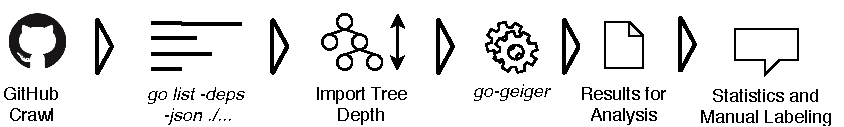
\includegraphics[width=\textwidth]{assets/figures/study-methodology.pdf}
    \caption{Overview of our Study Methodology}
    \label{fig:study-methodology}
\end{figure}


In the following, we first describe our evaluation data set and then provide in-depth analyses of \unsafe{} usage in the wild using \toolUsage{}.
% of how prevalent \unsafe{} is in the wild, in which way and why it is used in our test data set.
Our evaluation scripts as well as the results are available online\footnote{\url{https://github.com/stg-tud/unsafe_go_study_results}}.
%for further research.


%% included here for manual positioning one page earlier. Belongs to next section, reposition if needed
\begin{figure*}[!t]
    \vspace{2mm}
    \centering
    %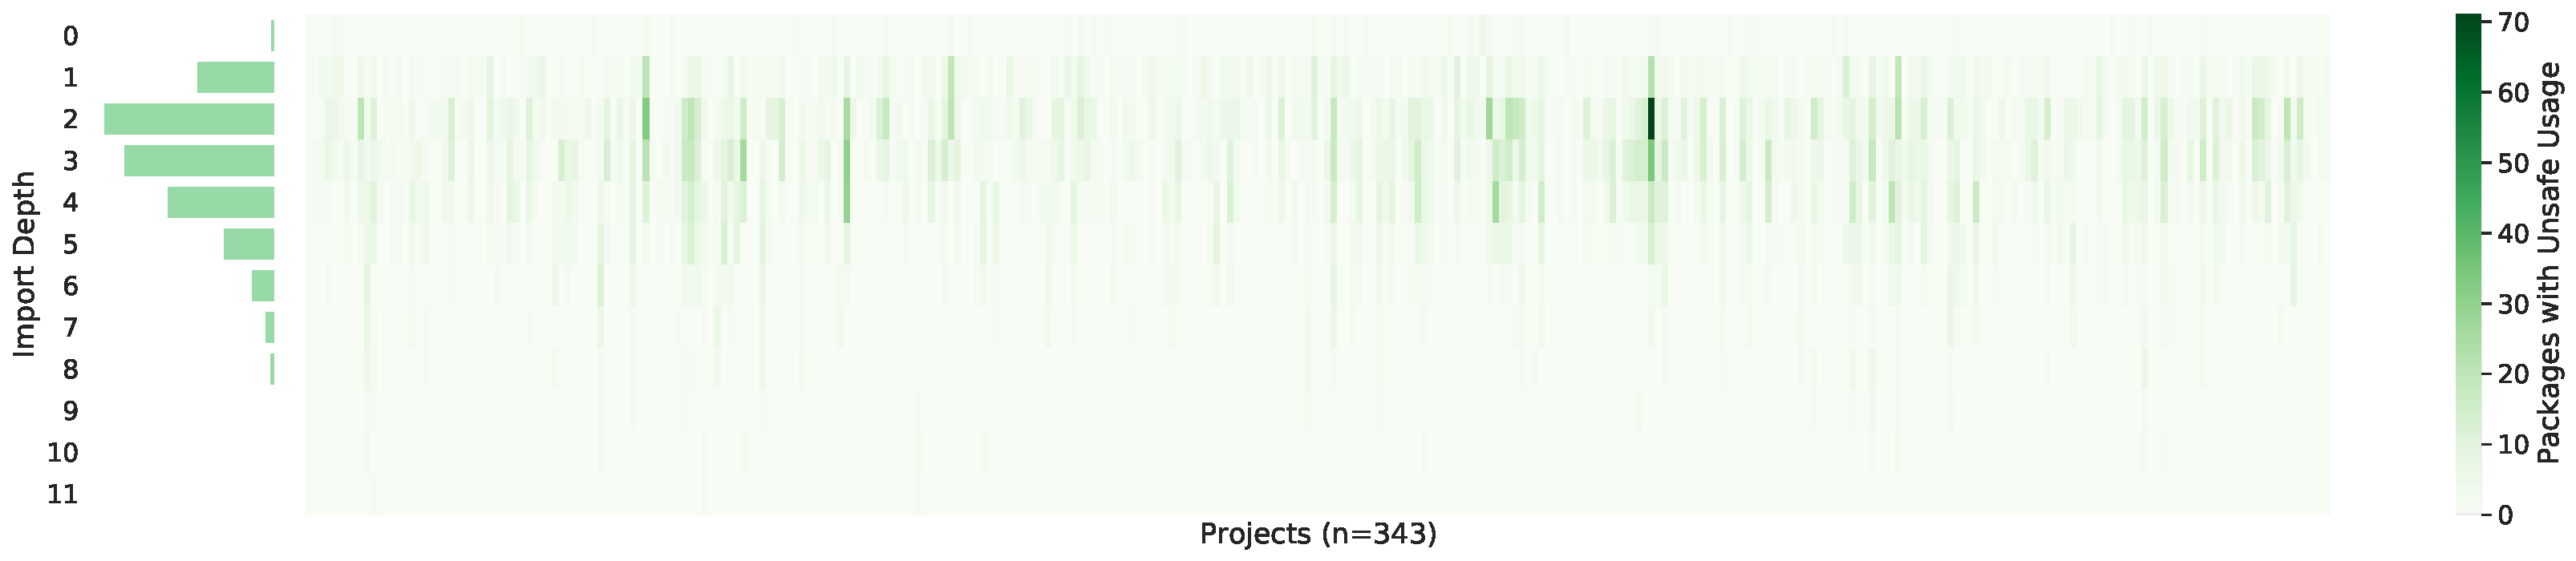
\includegraphics[width=\textwidth]{gfx/figures/unsafe-import-depth.pdf}
    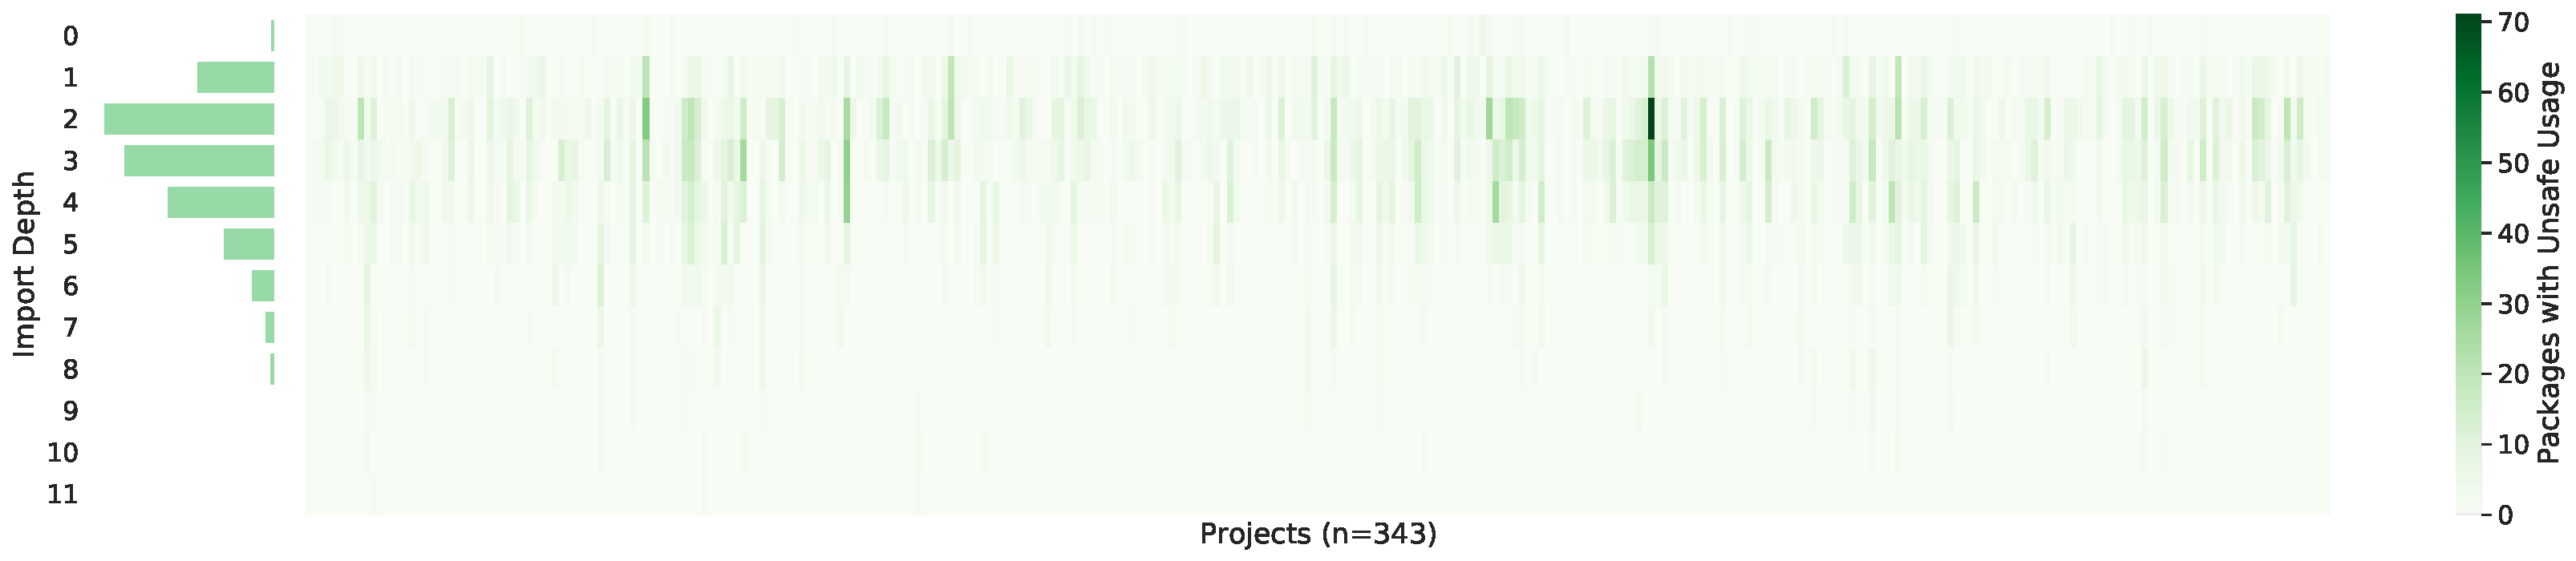
\includegraphics[width=.9\textwidth]{gfx/figures/unsafe-import-depth.pdf}
    \caption{Import Depth of Unsafe Packages. Unsafe packages are around a depth of \averageUnsafeImportDepth{} (sd=\stdUnsafeImportDepth{})}
    \label{fig:unsafe-import-depth}
    %\vspace{-10pt}
\end{figure*}




%% ---------------------------------------------------

\subsection{Data Set}

%For our evaluation, we created a data set of open-source Go code available on GitHub.
As our research is focused on open-source projects, we crawled the \initalProjs{} most-starred Go projects available on GitHub. 
To further understand the influence of dependencies, we then selected the applications supporting \textit{go modules}.
With the introduction of Go \checkNum{1.13}, \textit{go modules}\footnote{\url{https://blog.golang.org/using-go-modules}} are the official way to include dependencies.
Unfortunately, \withoutModules{} of the projects did not yet support Go modules.
Thus, we excluded them from our set.
Furthermore, \notCompiled{} projects that did not compile were also removed.
As a result, we ended up with \projsAnalyzed{} top-rated Go projects. % collected from GitHub.
These have between 72,988 and 3,075 stars, with an average of 7,860. % and median of 5,345. %, thus, this evaluation focuses on very popular projects.
%and save all findings into CSV files.



%% ---------------------------------------------------

\subsection{Unsafe Usages in Projects and Dependencies}
\label{sec:eval:unsafewild}

We used the Go tool chain to identify the root module of each project. 
This is the module defined by the top-level \textit{go.mod} file in the project.
Then we enumerated the dependencies of the project, and build the dependency tree.
For each package, we used \toolUsage{} to generate CSV reports of the found \unsafe{} usages.
Through these analyses we answer the research questions of how many projects use \unsafe{} either in their own code or dependencies (\ref{rq:prevalApp}), and how deep in the dependency tree are the most \unsafe{} code usages (\ref{rq:depsDepth}). 
By selecting only results from the project root modules, we can easily find out how many applications contain a first-hand use of \unsafe{} code.
Our data shows that \checkNum{131} (\checkNum{38.19\%}) projects have at least one \unsafe{} usage within the project code itself.
By looking closer at the imported packages, we see that \checkNum{3,388} of \checkNum{62,025} (\checkNum{5.46\%}) transitively imported packages use \unsafe{}. 
%Through filtering the imported packages, we find that \checkNum{33} of \checkNum{186} (\checkNum{17.74\%}) used standard library packages contain \unsafe{}.
%There are \checkNum{299} (\checkNum{87.17\%}) projects that have at least one direct dependency to a package that has $\geq 1$ unsafe dependency, however for this number we counted only packages belonging to the project's root module as first-party project code. \jl{Might be wrong numbers}
%If a project is split into several modules that all should be logically viewed as first-party project code, they will inflate this number.
There are \checkNum{312} (\checkNum{90.96\%}) projects that have at least one non-standard-library dependency with \unsafe{} usages somewhere in their dependency tree.
Since all projects include the Go runtime, which uses \unsafe{}, counting it as an \unsafe{} dependency would mean that \checkNum{100\%} of projects transitively include \unsafe{}.
We consider this to be less meaningful, as we assume the Go standard library is well audited and safer to use.

%\begin{tcolorbox}[boxsep=1pt, enlarge top by=5pt, title=Answer to \ref{rq:prevalDeps}]
\begin{tcolorbox}[boxsep=1pt, enlarge top by=5pt, title=Answer to \ref{rq:prevalApp}]
About \checkNum{38\%} of projects directly contain \unsafe{} usages.
Furthermore, about \checkNum{91\%} of projects transitively import at least one dependency that contains \unsafe{}.
\end{tcolorbox}

% Using this tree, we can identify the import depth as minimum depth in the tree for each package.
Figure~\ref{fig:unsafe-import-depth} shows the number of packages with at least one \unsafe{} usage by their depth in the dependency tree for every project on its own as a heatmap, alongside the distribution for all projects combined as bars on the left side.
It is evident that most packages with \unsafe{} are imported early in the dependency tree with an average depth of \averageUnsafeImportDepth{}~and a standard deviation of \stdUnsafeImportDepth{}.
This number is very similar to the overall average depth of imported packages (\averageGeneralImportDepth{}). %, regardless of whether they contain usages of \unsafe{}.
While the packages containing \unsafe{} can be manually found and evaluated, this process requires significant resources to handle the increasing number of packages introduced through each dependency. 
For developers only the first level of dependencies, the ones they added themselves, are really obvious.
On this level, \levelOneImportedUnsafePackagesCount{} out of \ImportedUnsafePackagesCount{} imported packages (\levelOneImportedUnsafePackagesShare{}) contain \unsafe{}.

\begin{tcolorbox}[boxsep=1pt, enlarge top by=5pt, title=Answer to \ref{rq:depsDepth}]
Most imported packages containing \unsafe{} usages are found around a depth of \checkNum{3} in the dependency tree.
\end{tcolorbox}



%% ---------------------------------------------------

\subsection{Types and Purpose of Unsafe in Practice}
\label{sec:eval:labeledData}

This section answers \ref{rq:distTypes} and \ref{rq:purpose}.
%This section answers the research questions which \unsafe{} keywords are used most (\ref{rq:distTypes}), as well as which \unsafe{} operations are used in practice for what purpose (\ref{rq:purpose}).
%
Figure~\ref{fig:unsafe-tokens-distribution} shows the distribution of the different \unsafe{} types in our data set.
Packages that are imported in different versions by the projects are counted once per version, as they might contain different \unsafe{} usages and coexist in the wild.
%We found various different usages of \unsafe{} in the analyzed projects, 
In our data set \textit{uintptr} and \textit{unsafe.Pointer} are used about equally often and by far the most common with almost 100,000 findings. 
Next, \textit{unsafe.Sizeof} is still used a bit ($\sim 3,700$), while the other \unsafe{} types are rarely used~($< 1,000$).

\begin{tcolorbox}[boxsep=1pt, enlarge top by=5pt, title=Answer to \ref{rq:distTypes}]
In the wild, \textit{uintptr} and \textit{unsafe.Pointer} are orders of magnitude more common than other \unsafe{} usages.
\end{tcolorbox}

\begin{figure}[!t]
    \centering
    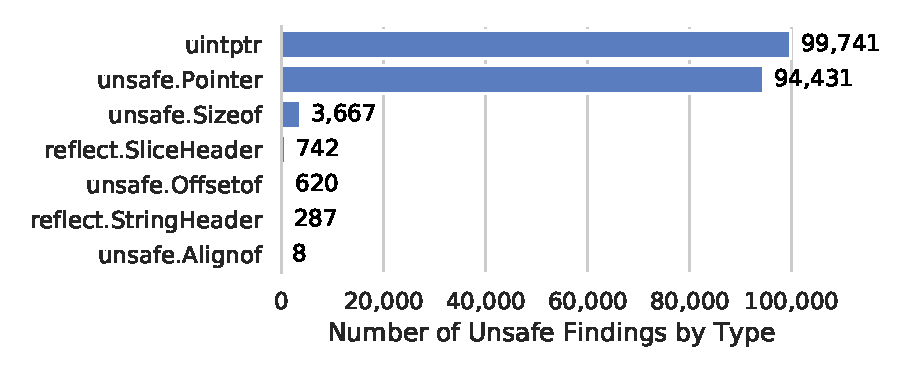
\includegraphics[width=0.43\textwidth]{assets/plots/distribution-unsafe-types.pdf}
    \caption{Distribution of different types of unsafe tokens}
    \label{fig:unsafe-tokens-distribution}
\end{figure}

To learn about the purpose and context in which \unsafe{} is used, we needed to manually analyze code.
Thus, we selected the top \checkNum{10} projects (Table~\ref{tbl:dataset-projects}) with the most \unsafe{} usages in non-standard library packages.
%These projects including the Git revision analyzed plus some additional data are shown in Table~\ref{tbl:dataset-projects}.
From these projects and all their transitive dependencies, we randomly sampled \checkNum{400} code snippets that were found in the \textit{standard library (std)} and \checkNum{1,000} snippets from the remaining packages (\textit{app}).
We define standard library code as all packages that are part of the Go standard library or the \textit{golang.org/x/sys} module, as the \textit{syscall} standard library package is deprecated in favor of this module\footnote{\url{https://golang.org/pkg/syscall}}.
We split the snippets into two groups to analyze if there is a difference between the official standard library and non-standard library code regarding the usage of \unsafe{}.
Then, we identify class labels in two dimensions: what is being done, and for what purpose. 
Finally, we manually analyze all \checkNum{1,400} code snippets and label them accordingly.
The results of this process are shown in Table~\ref{tbl:dataset-classes}.

\begin{table}[!t]
\vspace{2mm}

    \centering
    \caption{Projects selected for labeled data set}
    \label{tbl:dataset-projects}
    \begin{adjustbox}{max width=\textwidth}
    \begin{tabular}{llrrl}
        %\hline
        {} & \textbf{Name} &  \textbf{Stars} &  \textbf{Forks} &    \textbf{Revision} \\ \hline
        \rowcolor{verylightgray}
        1  &         kubernetes/kubernetes &  66,512 &  23,806 &  \texttt{fb9e1946b0} \\
        2  &                 elastic/beats &   8,852 &   3,207 &  \texttt{df6f2169c5} \\
        \rowcolor{verylightgray}
        3  &             gorgonia/gorgonia &   3,373 &    301 &  \texttt{5fb5944d4a} \\
        4  &              weaveworks/scope &   4,354 &    554 &  \texttt{bf90d56f0c} \\
        \rowcolor{verylightgray}
        5  &  mattermost/mattermost-server &  18,277 &   4,157 &  \texttt{e83cc7357c} \\
        6  &               rancher/rancher &  14,344 &   1,758 &  \texttt{56a464049e} \\
        \rowcolor{verylightgray}
        7  &                 cilium/cilium &   5,501 &    626 &  \texttt{9b0ae85b5f} \\
        8  &                     rook/rook &   7,208 &   1,472 &  \texttt{ff90fa7098} \\
        \rowcolor{verylightgray}
        9  &             containers/libpod &   4,549 &    539 &  \texttt{e8818ced80} \\
        10 &                       xo/usql &   5,871 &    195 &  \texttt{bdff722f7b} \\ %\hline
    \end{tabular}
    \end{adjustbox}
    %% reduce space after table for vspace tweaking
    \vspace{-10pt}
\end{table}
\begin{table*}[htp!]
    \centering
    \caption[Labeled unsafe.Pointer usages in application code (non standard library) and standard library samples]
        {Labeled unsafe.Pointer usages in application code (non standard library) and standard library samples~\newline \tiny ~\newline \footnotesize
        \underline{eff}: efficiency, \underline{ser}: (de)serialization, \underline{gen}: generics,
        \underline{no GC}: avoid garbage collection, \underline{atomic}: atomic operations,
        \underline{FFI}: foreign function interface, \underline{HE}: hide from escape analysis, \underline{layout}: memory layout control,
        \underline{types}: Go type system,
        \underline{reflect}: type reflection, \underline{unused}: declared but unused \tiny ~\newline}
    \label{tbl:dataset-classes}
    \begin{adjustbox}{max width=\textwidth}
    
    %% do not paste from notebook, local changes done!
\begin{tabular}{r|cc|cc|cc|cc|cc|cc|cc|cc|cc|cc|cc|cc}
                    & \multicolumn{2}{c|}{\textbf{eff}} & \multicolumn{2}{c|}{\textbf{ser}} & \multicolumn{2}{c|}{\textbf{gen}} & \multicolumn{2}{c|}{\textbf{no GC}} & \multicolumn{2}{c|}{\textbf{atomic}} & \multicolumn{2}{c|}{\textbf{FFI}} & \multicolumn{2}{c|}{\textbf{HE}} & \multicolumn{2}{c|}{\textbf{layout}} & \multicolumn{2}{c|}{\textbf{types}} & \multicolumn{2}{c|}{\textbf{reflect}} & \multicolumn{2}{c|}{\textbf{unused}} & \multicolumn{2}{c}{\textbf{total}} \\ %\hline
                    &  \textbf{app} &  \textbf{std} &  \textbf{app} &  \textbf{std} &  \textbf{app} &  \textbf{std} &   \textbf{app} &  \textbf{std} &    \textbf{app} &  \textbf{std} &  \textbf{app} &  \textbf{std} &  \textbf{app} &  \textbf{std} &    \textbf{app} &  \textbf{std} &   \textbf{app} &  \textbf{std} &     \textbf{app} &  \textbf{std} &    \textbf{app} &  \textbf{std} &   \textbf{app} &  \textbf{std} \\ \hline
                    
                    \textbf{cast} & 562 & 16 & 178 & 33 & 18 & & & & & & 24 & 6 && 2 & 3 & 13 & & 45 & 1 & & & & 786 & 115 \\ 
      %  cast-struct &  401 &    4 &   50 &    6 &    6 &      &       &      &        &      &    6 &    2 &      &    2 &        &    4 &       &   31 &         &      &        &      &   463 &   49 \\
%\rowcolor{verylightgray}
      %   cast-basic &   90 &    2 &   29 &    3 &    1 &      &       &      &        &      &    1 &    3 &      &      &      2 &    7 &       &    1 &         &      &        &      &   123 &   16 \\
      %  cast-header &   36 &    1 &    3 &      &    1 &      &       &      &        &      &      &      &      &      &        &      &       &    3 &         &      &        &      &    40 &    4 \\
%\rowcolor{verylightgray}
      %   cast-bytes &   22 &    1 &   81 &   11 &      &      &       &      &        &      &    1 &      &      &      &      1 &      &       &    1 &         &      &        &      &   105 &   13 \\
      % cast-pointer &   13 &    8 &   15 &   13 &   10 &      &       &      &        &      &   16 &    1 &      &      &        &    2 &       &    9 &       1 &      &        &      &    55 &   33 \\
\rowcolor{verylightgray}
      \textbf{memory-access} &    2 &    1 &    9 &      &      &      &       &      &        &      &      &    1 &      &      &      4 &    6 &       &    4 &         &      &        &      &    15 &   12 \\
 \textbf{pointer-arithmetic} &    7 &    2 &    6 &    1 &      &      &       &      &        &    1 &      &    3 &    1 &    2 &      3 &    8 &       &    9 &         &      &        &      &    17 &   26 \\
\rowcolor{verylightgray}
         \textbf{definition} &    4 &    1 &   23 &      &    2 &      &       &      &        &      &    4 &    5 &      &      &        &    9 &       &    8 &       6 &    3 &        &      &    39 &   26 \\
           \textbf{delegate} &    4 &      &   64 &      &    2 &      &       &      &     11 &    5 &   29 &   45 &      &    4 &        &   14 &       &    6 &         &    1 &        &      &   110 &   75 \\
\rowcolor{verylightgray}
            \textbf{syscall} &      &      &      &      &      &      &    17 &  138 &        &      &      &      &      &      &        &      &       &      &         &      &        &      &    17 &  138 \\
             \textbf{unused} &      &      &      &      &      &      &       &      &        &      &      &      &      &      &        &      &       &      &         &      &     16 &    8 &    16 &    8 \\ \hline
%\rowcolor{verylightgray}
                  \textbf{total} &  579 &   20 &  280 &   34 &   22 &    0 &    17 &  138 &     11 &    6 &   57 &   60 &    1 &    8 &     10 &   50 &     0 &   72 &       7 &    4 &     16 &    8 &  1000 &  400 \\
\end{tabular}

    \end{adjustbox}
        \vspace{-10pt}
\end{table*}

In the following, we outline the identified usage type classes describing what is being done in code.
The most prevalent are \textit{cast} operations from arbitrary types to other structs, basic Go types such as integers, slice/string headers, byte slices, or raw \textit{unsafe.Pointer} values. 
%The most prevalent are \textit{cast-struct}, \textit{cast-basic}, \textit{cast-header}, \textit{cast-bytes}, and \textit{cast-pointer}, which are all cast operations from arbitrary types to other arbitrary structs, basic Go types such as integers, slice or string headers, byte slices, or raw \textit{unsafe.Pointer} values.
The \textit{memory-access} class is applied where \textit{unsafe.Pointer} values are dereferenced, used to manipulate corresponding memory or for comparison with another address.
\textit{Pointer-arithmetic} denotes usages of \unsafe{} to do some form of arithmetic manipulation of addresses, such as advancing an array.
\textit{Definition} groups usages where a field or method of type \textit{unsafe.Pointer} is declared for later usage.
\textit{Delegate} are instances where \unsafe{} is only needed in a function to pass it along to another function requiring a parameter of type \textit{unsafe.Pointer}. 
Thus, the need to use \unsafe{} is actually located elsewhere.
\textit{Syscall} are calls using the Go \textit{syscall} package or \textit{golang.org/x/sys} module.
As the name suggests, \textit{unused} is a class of occurrences that are not actually used in the analyzed code, e.g. dead code or unused parameters.

Our identified purpose classes, providing hints on why \unsafe{} is used, are described in the following.
\textit{Efficiency} includes cases where \unsafe{} is used only for the aim to improve time or space efficiency of the code.
The \textit{serialization} class contains (un)marshalling and (de)serialization operations such as in-place casts from complex types to bytes.
\textit{Generics} applies when \unsafe{} is used to build functionality that would otherwise be solved with generics if they were available in Go.
Samples in the \textit{avoid garbage collection} class are used to tell the Go compiler to not free a value while it is used, e.g., by a function written in assembly.
The \textit{atomic operations} class contains usages of the \textit{atomic} API which expects \unsafe{} for some functions.
The \textit{foreign function interface (FFI)} class contains interoperability with C code (CGo), and calling  functions that expect their parameters as \unsafe{} pointers.
\textit{Hide from escape analysis} includes the pattern described earlier (Listing~\ref{lst:unsafe-ex-escape-analysis}) to break the escape analysis chain.
The \textit{memory layout control} class contains code used for low-level memory management.
\textit{Types} snippets are used by the standard library to implement the Go type system.
\textit{Reflect} includes instances of type reflection and re-implementations of some types of the \textit{reflect} package, e.g. using \textit{unsafe.Pointer} instead of \textit{uintptr} for slice headers.
Again, \textit{unused} is a class of unused occurrences.

%Among the \checkNum{1,400} labeled snippets, \checkNum{683} are located in automatically generated code.
%It might be safe to assume that generated code is less dangerous, however, as bugs in the code generator can have very serious effects of scale, we included them in the study nonetheless.

Using \unsafe{} for the sake of efficiency is the most prevalent motivation to use \unsafe{} in the wild covering \checkNum{58\%} in application code, whereas it is only used for this purpose in \checkNum{5\%} of the cases in std. 
From these, \checkNum{97\%} resp. \checkNum{80\%} are achieved by casting different types. 
The second biggest reason to use \unsafe{} in app is to perform some form of (de)serialization, accounting for \checkNum{28\%}.
%Interestingly, we observe efficiency improvements for \checkNum{4\%} and \checkNum{58\%} of the usages for the standard library and the remaining libraries, respectively.
For the standard library, the most relevant motivation is avoiding garbage collection with \checkNum{35\%}, whereas this is only used in \checkNum{2\%} of the usages in the app sample.
Furthermore, in std type \checkNum{18\%}, FFI \checkNum{15\%} and memory layout \checkNum{13\%} related \unsafe{} usages are rather common.
Both subsets share that hiding from escape analysis with \checkNum{0.1\%} (\textit{app}) and \checkNum{2\%} (\textit{std}) and using \unsafe{} for reflection with \checkNum{1\%} (both) are rare.
%Another interesting observation is that there seem to be two main motivations which occur only for the standard- or 3rd party libraries respectively. 
%Only the standard library makes use of \unsafe{} to implement types being \checkNum{5\%} of the analyzed code snippets. 
%All usages (\checkNum{2\%}) to solve the missing generics functionality in Go are within 3rd party libraries. 
Implementation of generics functionality which is currently missing in Go is only done in few samples (\checkNum{2\%}), although some of the finding in the serialization class could alternatively be achieved with generics as well.

%It is obvious that most of the \unsafe{} found in the wild is used to improve efficiency by casting different types in place, or for fast (un)marshalling operations that would otherwise need either reflection or support for generics.
%Furthermore, \unsafe{} is required to call some functions that expect it, such as atomic operations or certain \textit{FFI} functions.
%The standard library makes extensive use of \unsafe{} to implement types and memory management.
%Hiding values from escape analysis on purpose is done rarely.

\begin{tcolorbox}[boxsep=1pt, enlarge top by=5pt, title=Answer to \ref{rq:purpose}]
\checkNum{More than half} of the \unsafe{} usages in projects and 3rd party libraries are to improve efficiency via \unsafe{} casts.
In the Go standard library, \checkNum{every third} use of \unsafe{} is to avoid garbage collection. 
\end{tcolorbox}


\subsection{Vulnerable Usages}
\label{sec:discussion}
Looking at the study results, we see that \unsafe{} is used consistently and wide-spread in the most popular open-source Go projects.
One might argue that the patterns found by \toolUsage{} are only minor annoyances, not severe or would require a manual case-to-case inspection. 
The exploitability of several of these patterns was discussed in Section~\ref{sec:appr} with a link to proof-of-concept exploit code that we developed, clearly showing that it is indeed possible to use the memory corruptions to one's advantage.
However, not all \unsafe{} usages contain a vulnerability. 
As already discussed, we implemented more specific checks for some of our patterns known to be problematic in \toolSA{}.
The application of \toolSA{} to our data set revealed more than \numberBugsFixed{} bugs in different projects.
Based on the results, we submitted so far \numberPRs{} pull requests to fix the found bugs. %, which focuses on a subset of vulnerable code patterns.
By now, \numberPRsMerged{} have already been reviewed, acknowledged, and accepted by the corresponding project maintainers.
\section{Threats to Validity}
\label{sec:threatsToValidity}

%Since we showed actual exploit vectors and bugs with code snippets that are commonly used in popular real-world applications, we think that research on \unsafe{} is clearly not only an academic issue, but has direct and important consequences on the actual software market.
%Audit efforts should be made up to an import depth of around 4.


Potential internal threats to validity for our study include bias towards bigger projects because those might be over-represented in the manually labeled data set. 
External threats include a bias towards more active projects with many developers because we selected a subset of the most-starred open-source projects on GitHub. 
Also we only considered projects that use the Go module system and about a third of the top 500 projects are not covered by the analysis yet.
Further, we could have missed projects from a special domain not having that many stars which might have other usage scenarios for \unsafe{} Go.
Nevertheless, one can argue that the biggest projects also have professional developers, higher standards and code gets more reviewed, thus, code quality should be higher.


\section{Related Work}
\label{sec:rw}

Empirical studies on unsafe code blocks in Rust projects: Qin \cite{qin2020} and Evans \cite{evans2020}.
Qin analyzed the Git history and focused on confirmed bugs and vulnerabilities.
Evans focused on search and discovery by static code analysis, like we did.
Escape analysis: Wang \cite{wang2020}. They actively use the pattern we identified as bug in many projects to hide variables from escape analysis in order to perform static code optimization.
Bug finder tools usability: \cite{smith2020}. The authors recommend integrated error messages in the IDE (future work?), contextualized and meaningful notifications, and good integration into CI.
Counting dependencies that matter: Pashchenko \cite{pashchenko2018}. Study on Maven / Java but results applicable to Go.
Exclude testing dependencies: we can't do that, but we exclude test files.
For package popularity count the projects that transitively include the package.
Problem: if a third-party library depends on an unsafe library, then we cannot simply update that library but instead we must wait for the third-party library to update or switch libraries.
We contribute an analysis of import depth.
Dependency update: Kula \cite{kula2017} finds that dependencies are often updated slowly or never. Mirhosseini \cite{mirhosseini2017}: automated PRs or badges can help, and a single bad experience in updating (breaking code) can make developers be reluctant to updates for a long time.
Go concurrency bugs: Tu \cite{tu2019} present a study on Go concurrency bugs. They also identified bugs with commit messages, which we did not do.
\todo{Unsafe Study for Java}

\section{Conclusion}
\label{sec:concl}

We conducted the first (to the best of our knowledge) empirical study on the use of \unsafe{} Go code in the wild.
We find that ...

% conference papers do not normally have an appendix

% use section* for acknowledgment
\ifCLASSOPTIONcompsoc
  % The Computer Society usually uses the plural form
  %\section*{Acknowledgments}
\else
  % regular IEEE prefers the singular form
  %\section*{Acknowledgment}
\fi

This work has been funded by the German Federal Ministry of Education and Research and
the Hessen State Ministry for Higher Education, Research and the Arts within their joint support of
the National Research Center for Applied Cybersecurity ATHENE.


% trigger a \newpage just before the given reference
% number - used to balance the columns on the last page
% adjust value as needed - may need to be readjusted if
% the document is modified later
%\IEEEtriggeratref{8}
% The "triggered" command can be changed if desired:
%\IEEEtriggercmd{\enlargethispage{-5in}}

% references section

% can use a bibliography generated by BibTeX as a .bbl file
% BibTeX documentation can be easily obtained at:
% http://mirror.ctan.org/biblio/bibtex/contrib/doc/
% The IEEEtran BibTeX style support page is at:
% http://www.michaelshell.org/tex/ieeetran/bibtex/
\bibliographystyle{IEEEtran}
\balance
\bibliography{IEEEabrv,references, references-withoutZotero}

% that's all folks
\end{document}
